\documentclass[11pt]{aghdpl}
% \documentclass[en,11pt]{aghdpl}  % praca w języku angielskim
\usepackage[polish]{babel}
%\usepackage[english]{babel}
\usepackage[utf8]{inputenc}
\usepackage[T1]{fontenc}

% dodatkowe pakiety
\usepackage{enumerate}
\usepackage{listings}
\lstloadlanguages{TeX}

\usepackage{listings}
\usepackage{xcolor}
\definecolor{listinggray}{gray}{0.9}
\definecolor{lbcolor}{rgb}{0.9,0.9,0.9}
\lstset{
    backgroundcolor=\color{lbcolor},
    tabsize=4,
  language=C++,
  captionpos=b,
  tabsize=3,
  frame=lines,
  numbers=left,
  numberstyle=\tiny,
  numbersep=5pt,
  breaklines=true,
  showstringspaces=false,
  basicstyle=\footnotesize,
%  identifierstyle=\color{magenta},
  keywordstyle=\color[rgb]{0,0,1},
  commentstyle=\color{Darkgreen},
  stringstyle=\color{red}
  }
\lstset{
  literate={ą}{{\k{a}}}1
           {ć}{{\'c}}1
           {ę}{{\k{e}}}1
           {ó}{{\'o}}1
           {ń}{{\'n}}1
           {ł}{{\l{}}}1
           {ś}{{\'s}}1
           {ź}{{\'z}}1
           {ż}{{\.z}}1
           {Ą}{{\k{A}}}1
           {Ć}{{\'C}}1
           {Ę}{{\k{E}}}1
           {Ó}{{\'O}}1
           {Ń}{{\'N}}1
           {Ł}{{\L{}}}1
           {Ś}{{\'S}}1
           {Ź}{{\'Z}}1
           {Ż}{{\.Z}}1
}



%\usepackage[pdftex]{graphicx}
\usepackage{tikz}
%---------------------------------------------------------------------------

\author{Żaneta Błaszczuk, Rafał Kozik, Filip Kubicz, Jakub Nowak, Jakub Porębski}
\shortauthor{Ż. Błaszczuk, R. Kozik, F. Kubicz, J. Nowak, J. Porębski}

\titlePL{Podwójne wahadło}
\titleEN{Double pendulum}

\shorttitlePL{Podwójne wahadło} % skrócona wersja tytułu jeśli jest bardzo długi
%\shorttitleEN{Thesis in \LaTeX}

\thesistype{Modelowanie układów fizycznych i biologicznych}
%\thesistype{Master of Science Thesis}

\supervisor{dr inż. Ireneusz Wochlik}

\degreeprogramme{Automatyka i Robotyka}
%\degreeprogramme{Computer Science}

\date{2014}

\department{Katedra Automtyki}
%\department{Department of Applied Computer Science}

\faculty{Wydział Elektrotechniki, Automatyki,\protect\\[-1mm] Informatyki i Inżynierii Biomedycznej}
%\faculty{Faculty of Electrical Engineering, Automatics, Computer Science and Biomedical Engineering}

\setlength{\cftsecnumwidth}{10mm}

\begin{document}
\titlepages

\section{Teoria}
Wahadło podwójne jest to wahadło matematyczne zawieszone na drugim wahadle matematycznym. Jego schemat pokazuje rys. \ref{Schemat}.
\begin{figure}[h!]
\centering
\label{Schemat}
\setlength{\unitlength}{2mm}
\begin{picture}(50,35)(0,15)

\put(25,50){\vector(1,0){3}}
\put(25,50){\vector(0,-1){3}}
\put(27,49){\makebox(0,0){$x$}}
\put(24,48){\makebox(0,0){$y$}}

\put(20,50){\line(1,0){10}}
\multiput(25,48)(0,-2){7}{\line(0,1){1}}
\put(25,50){\line(1,-3){5}}
\put(30,35){\circle*{2}}

\put(27,38){\makebox(0,0){$\varphi_1$}}
\put(30,40){\makebox(0,0){$l_1$}}
\put(33,35){\makebox(0,0){$m_1$}}

\multiput(30,33)(0,-2){7}{\line(0,1){1}}
\put(30,35){\line(1,-5){4}}
\put(34,15){\circle*{2}}

\put(31.5,22){\makebox(0,0){$\varphi_2$}}
\put(33,25){\makebox(0,0){$l_2$}}
\put(37,15){\makebox(0,0){$m_2$}}

\end{picture}
\caption{Schemat wahadła}
\end{figure}
Wahadło opisuje 5 parametrów masy $m_1$ i $m_2$, długości $l_1$ i $l_2$ oraz przyśpieszenie ziemskie $g$. Można jednka zmniejszyś ich ilość podstawiając: 
\begin{equation}
	A = \frac{m_1}{m_2} \qquad B = \frac{l_2}{l_1} \qquad C = \frac{g}{l_1}
\end{equation}
Stan wahadł opisują cztery parametry: kąty $\varphi_1$ i $\varphi_2$ oraz prędkości kątowe $\omega_1$ i $\omega_2$. 
Ruch opisuje układ czterech równań różniczkowych:
\begin{equation}
	\dot{\varphi}_1 = \omega_1
\end{equation}
\begin{equation}
	\dot{\omega}_1=-\frac{\sin(\varphi_1-\varphi_2)(B\omega_2^2+\omega_1^2cos(\varphi_1-\varphi_2))+C((A+1)\sin(\varphi_1)-
	\sin(\varphi_2)cos(\varphi_1-\varphi_2))}{A+\sin^2(\varphi_1-\varphi_2)}
\end{equation}
\begin{equation}
	\dot{\varphi}_2 = \omega_2
\end{equation}
\begin{equation}
	\dot{\omega}_2 = \frac{(A+1)(\omega_1^2\sin(\varphi_1-\varphi_2)-C\sin(p2))+\cos(\varphi_1-\varphi_2)((B\omega_2^2 \sin(\varphi_1-\varphi_2))+C(A+1)\sin(\varphi_1))}{B(A+\sin^2(\varphi_1-\varphi_2))}
\end{equation}
W modelu nie uwzględniono tarcia.
\section{Implementacja}
Równiania zostały rozwiązane numerycznie za pomocą metody Rungego-Kutty czwartego rzędu która została zaimplementowana w języku c++. Wyniki zostały zapisane do pliku tekstowego, w każdej lini odzielone spacjami: czas od początku symulacji, kąty $\varphi_1$, $\varphi_2$ oraz prędkości kątowe $\omega_1$ i $\omega_2$. Wykeresy zostały przygotowane w programie gnuplot. Powstał także program przedstawiający ruch wahadła napisany z wykorzystaniem biblioteki QT. Wygląd programu pokazuje rys. \ref{QTgui}. Kody źródłowe przygotowanego oprogramowania znajdują się w repozytorium pod adresem www.github.com/Qbicz/MUFB. 

\begin{figure}[h!]
	\centering
	\label{QTgui}
	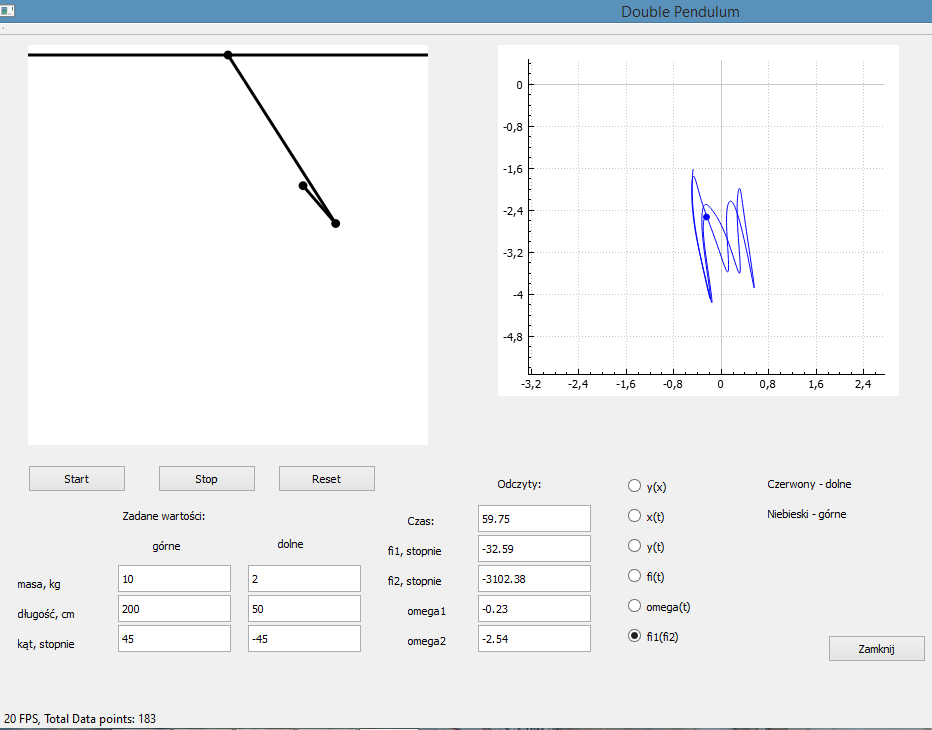
\includegraphics[width=0.4\textwidth]{qtgui.png}
	\caption{Graficzna symulacja ruchu wahadła.}
\end{figure}

\section{Wyniki}
Symulacja dla parametrów $A = 100$, $B = 1$, $C = 1$ oraz stanu w chwili $t_0=0$ $\varphi_1(0) = 0$, $\varphi_2(0) = 1$, $\omega_1(0) = 0$ i $\omega_2(0) = 0$. Symulacja trwała 300 sekund z krokiem co 0,001 sekundy.  \\
Rys. \ref{phi1_2odt.} przedstawia wartości kątów $\varphi_1$, $\varphi_2$, $\omega_1$ oraz $\omega_2$ w funkcji czasu. Dla tak dobranych parametrów powstają dudnienia.
\begin{figure}[h!]
	\centering
	\label{phi1_2odt.}
	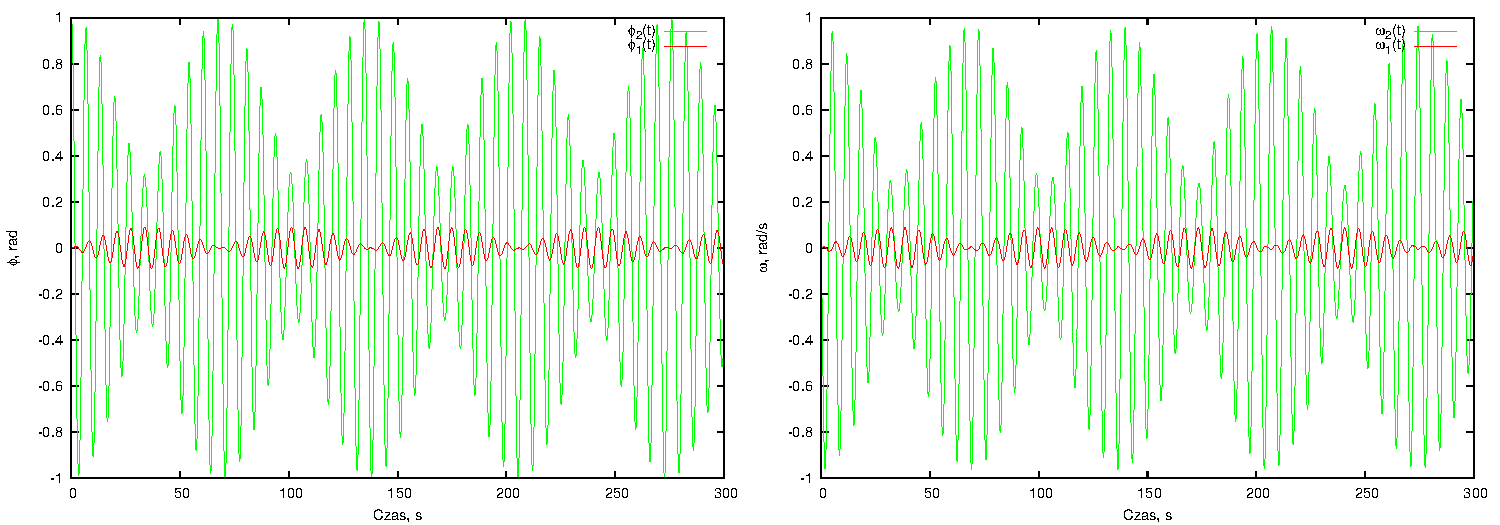
\includegraphics[width=0.95\textwidth]{phi1_2t.pdf}
	\caption{Kąty oraz prędkości kątowe w funkcji czasu.}
\end{figure}
Rys. \ref{phi1_phi2.} przedstawia trajektorię ruchu wahadła narysowaną w przestrzenie $\varphi_1$, $\varphi_2$. Dla 300 sekund nie da się zaobserwować żadnej regularnonści w ruchu wahadła.
\begin{figure}[h!]
	\centering
	\label{phi1_phi2.}
	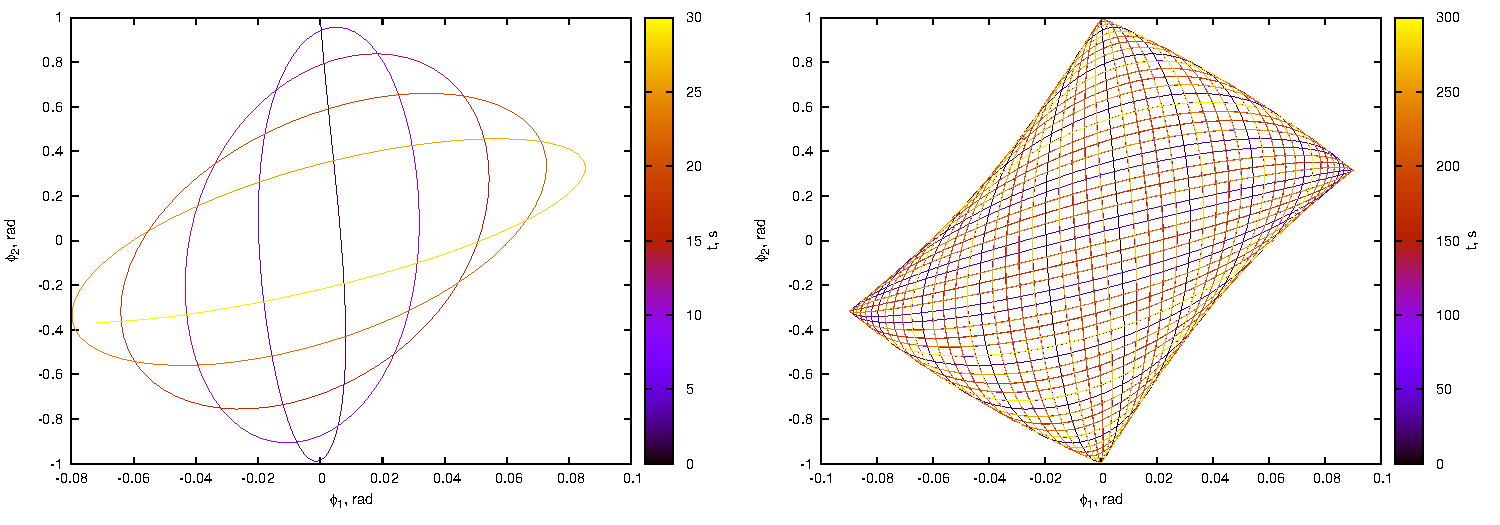
\includegraphics[width=0.95\textwidth]{phi1_phi2.pdf}
	\caption{Trajektoria w przestrzenie $\varphi_1$, $\varphi_2$ a) dla pierwszych 30 sekund i b) dla 300 sekund.}
\end{figure}
Rys. \ref{phi_omega} przedstawia trajektorie w przestrzeni fazowej: wykresy prędkości kątowej w funkcji wartości kąta.
\begin{figure}[h!]
	\centering
	\label{phi_omega}
	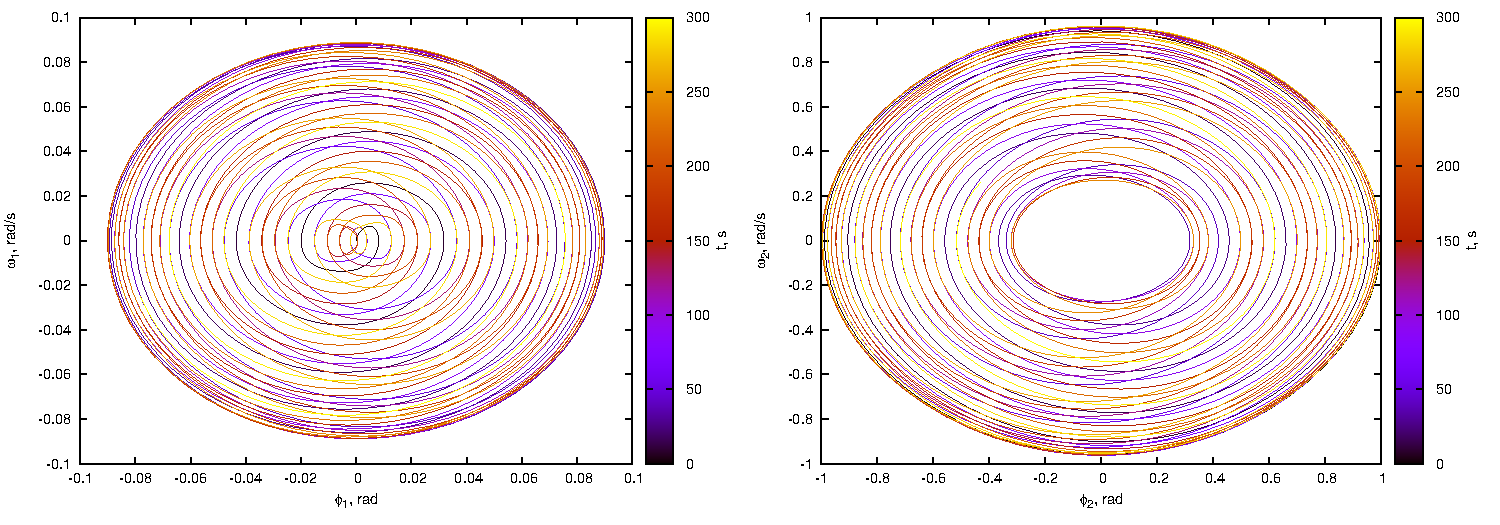
\includegraphics[width=0.95\textwidth]{phi1_omega1.pdf}
	\caption{Trajektoria w przestrzeni fazowej.}
\end{figure}




\section{Bibliografia}
1. Wróblewski J. praca licencjacka "Wahadło podwójne" Warszawa 2011\\
2.Dudek-Dyduch E., Wąs J., Dutkiewicz L., Grobel-Dębska K., Gudowski B. "Metody numeryczne wybrane zagadnienia" Wydawnictwo AGH Kraków 2011 

\end{document}